\section{Checkpointing} \label{sec:bg-checkpointing}
In this section, I will show how peak memory occurs during neural network training and show how to reduce this using checkpointing.
% The first key behind all memory optimisations using this graph is that the entire training process is this exact same step repeated many times.
% Thus, even though training may take days or even weeks [?], we only have to optimise a relatively small computational graph.
% Compared to the time taken for a single training step, we can spend a huge amount of time solving for the best optimisation strategies; it only has to be fast relative to the entire training process.

\subsection{Analysing Memory Usage During Training}
Recall the computational graph for one step of training a neural network, repeated in Figure \ref{fig:2-nn-comp-graph-2}.

\begin{figure}[htb]
    \centering
    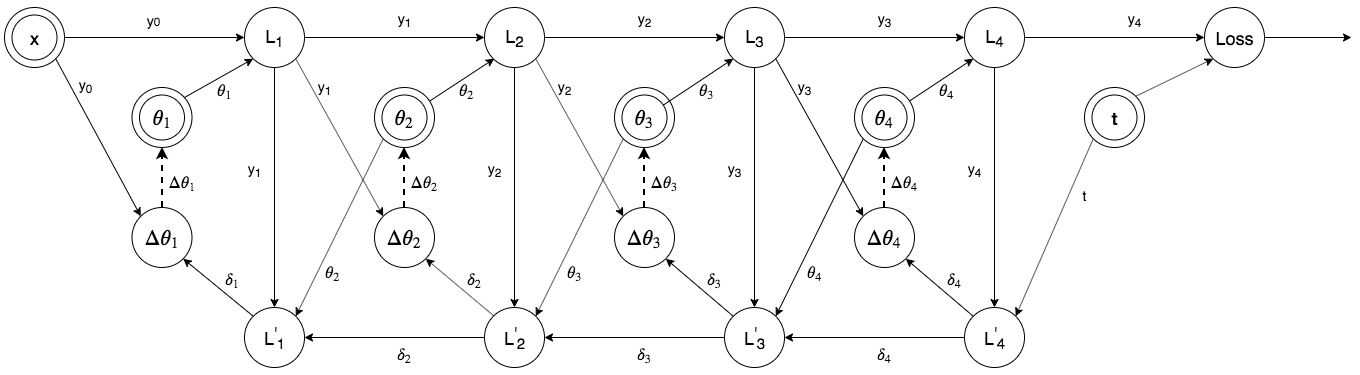
\includegraphics[width=0.97\linewidth]{backprop_full_comp_graph.png}
    \caption{The computational graph for one step of gradient descent on a neural network of four layers.}
    \label{fig:2-nn-comp-graph-2}
\end{figure}

We need to analyse what is actually consuming memory and what is the bottleneck. From the graph, we can see what needs to be allocated:
\begin{itemize}[topsep=0.1em]
    \item The forwards;
    \item The backwards;
    \item The weights;
    \item The targets.
\end{itemize}
However, there is some less obvious memory consumption too.
\begin{itemize}[topsep=0.1em]
    \item \textbf{Workspaces}: Different algorithms for an operator can have different memory requirements. The memory required for an algorithm is known as the workspace.
    \item \textbf{Additional Optimiser Memory}: As mentioned before, in practice vanilla SGD is not used much. Many of the other optimisers require extra memory than just the \(\Delta\theta\). For example they may smooth the update of a parameter by taking some average of the gradient and the previous gradients, in which case the previous gradient must be stored for every parameter.
    \item \textbf{Miscallenous}: The implementation used will likely allocate some miscallenous memory. Between versions of a framework, the exact configuration used, etc., it would be infeasible to account for this statically in a cost model.
\end{itemize}

In my implementation, I will account for the workspace memory as part of the memory required for the forwards and backwards operations.

\begin{figure}[htb]
    \centering
    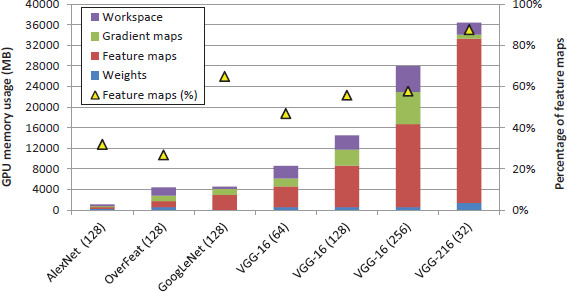
\includegraphics[width=0.7\linewidth]{network_memory_usage_breakdown.jpg}
    \caption{Breakdown of memory usage of popular networks. \cite[fig.~4]{Rhu2016}}
    \label{fig:2-memory-breakdown}
\end{figure}

I will not apply checkpointing to the weights or additional optimiser memory because they only use a small proportion of the total memory reqiurement.
Figure \ref{fig:2-memory-breakdown} shows a break down of memory consumption of popular network architectures.
As can be seen, the proportion of memory allocated to the weights is very small.
The reason is that modern deep networks hardly use fully-connected layers,
which cause an exponential growth in the number of weights.
Instead, we mostly see layers such as the convolutional layer \todo{put in bg}.
These typically apply a small filter, such as of size 3x3, to many large images. \todo{refs?}
The image is the forward tensor and the filter weights are the learnable parameters.
Thus the parameters are very small compared to the forward and backward tensors.
As the optimiser memory is usually equivalent to one or two extra values \textit{per parameter},
they are omitted from the optimisations too.
%targets? do i omitt them from optimisation, or are they profiled as part of final layer?

Therefore, we can omit the parameters from our analysis.
When checkpointing is applied, it will be assumed that the parameters and their gradients persist in memory throughout the forwards and backwards passes.
However, performing the backwards operators will still involve computing their updates, so the cost of this must be modelled.
The computational cost is modelled because solving for the optimal checkpointing policy requires the per-layer computational costs as well as the memory-costs, since it trades compute for memory.

Omitting the parameters from the computational graph in Figure \ref{fig:2-nn-comp-graph-2} results in the graph typically found in the literature, with some slight tweaks, shown in Figure \ref{fig:2-simplified-comp-graph}.

\begin{figure}[h]
    \centering
    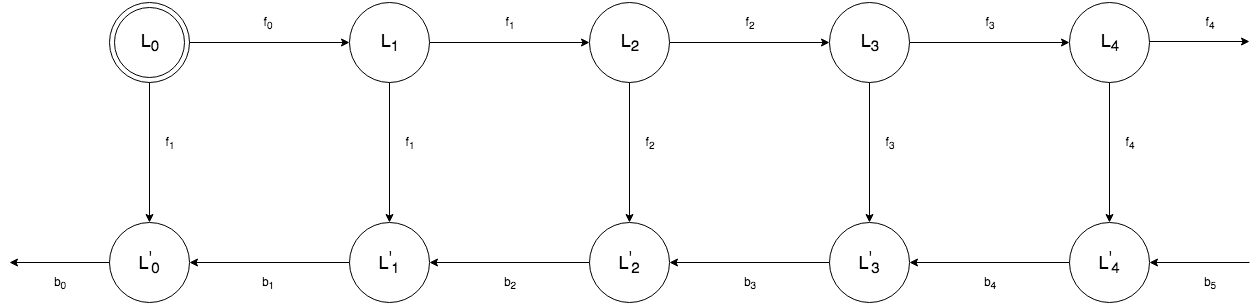
\includegraphics[width=0.9\linewidth]{simplified_comp_graph.png}
    \caption{Computational graph for one step of training, not showing the parameters or their gradients.}
    \label{fig:2-simplified-comp-graph}
\end{figure}

The loss node has also been omitted for brevity.

The forward operators \(L_i\) represent the same forward functions as before.
\(f_{i-1}\) is their input and \(f_{i}\) is their output.
The memory cost of \(f_i\) is modelled as all the (non-parameter) memory required to compute \(y_i\) in the original graph, including the workspace and \(y_i\) itself. The cost of computing \(f_i\) is just the cost of performing \(L_i\) to compute \(y_i\)

The backwards operators \(L^\prime_i\) have been defined differently to further simplify the graph. They perform two operations:
(i) using the output of layer \(y_i\) and the upstream backward \(\delta_{i+1}\), compute the upstream weight gradients \(\Delta\theta_{i+1}\); and
(ii) again using the output of layer \(y_i\) and the upstream backward \(\delta_{i+1}\), compute the downstream delta \(\delta_i\).
This means \(L^\prime_{i-1}\) will compute \(\Delta\theta_{i}\).
An \(L^\prime_0\) must then be added to the graph to represent the computation of \(\Delta\theta_0\).

The memory cost of \(b_i\) is thus all the memory required for \(\delta_i\), but not that for \(\Delta\theta_{i+1}\) as we have excluded parameter memory. However, the computational cost will include the cost to compute \(\Delta\theta_{i+1}\).

\(f_0\) is the inputs. For a network of \(N\) layers, \(f_N\) is the output of the network. \(b_{N+1}\) is the targets. \(b_0\) is not really a tensor that exists; it represents the output of \(L^\prime_{0}\), which is there to set \(\Delta\theta_0\), but does not actually output anything. However, as this incurs some computational cost, which will affect what strategy best optimises the network, we still model this `tensor'.

% need previous section on pebbling, in-place and sharing optimisations, state pytorch applies them aggressively
% in this section show how peak memory comes about (assuming pebbling)
% show how checkpointing gives O(2sqrt(n)) memory
% but no multiple recomps, no per-layer costs, and is arbitrary point on C-M curve
% show how to solve for this with uniform costs using DP
% give eqns, algo to solve.